%% Creator: Inkscape 0.91, www.inkscape.org
%% PDF/EPS/PS + LaTeX output extension by Johan Engelen, 2010
%% Accompanies image file 'Branch_Bound.pdf' (pdf, eps, ps)
%%
%% To include the image in your LaTeX document, write
%%   \input{<filename>.pdf_tex}
%%  instead of
%%   \includegraphics{<filename>.pdf}
%% To scale the image, write
%%   \def\svgwidth{<desired width>}
%%   \input{<filename>.pdf_tex}
%%  instead of
%%   \includegraphics[width=<desired width>]{<filename>.pdf}
%%
%% Images with a different path to the parent latex file can
%% be accessed with the `import' package (which may need to be
%% installed) using
%%   \usepackage{import}
%% in the preamble, and then including the image with
%%   \import{<path to file>}{<filename>.pdf_tex}
%% Alternatively, one can specify
%%   \graphicspath{{<path to file>/}}
%%
%% For more information, please see info/svg-inkscape on CTAN:
%%   http://tug.ctan.org/tex-archive/info/svg-inkscape
%%
\begingroup%
  \makeatletter%
  \providecommand\color[2][]{%
    \errmessage{(Inkscape) Color is used for the text in Inkscape, but the package 'color.sty' is not loaded}%
    \renewcommand\color[2][]{}%
  }%
  \providecommand\transparent[1]{%
    \errmessage{(Inkscape) Transparency is used (non-zero) for the text in Inkscape, but the package 'transparent.sty' is not loaded}%
    \renewcommand\transparent[1]{}%
  }%
  \providecommand\rotatebox[2]{#2}%
  \ifx\svgwidth\undefined%
    \setlength{\unitlength}{453.49843183bp}%
    \ifx\svgscale\undefined%
      \relax%
    \else%
      \setlength{\unitlength}{\unitlength * \real{\svgscale}}%
    \fi%
  \else%
    \setlength{\unitlength}{\svgwidth}%
  \fi%
  \global\let\svgwidth\undefined%
  \global\let\svgscale\undefined%
  \makeatother%
  \begin{picture}(1,0.34669268)%
    \put(0.05616224,0.32022762){\color[rgb]{0,0,0}\makebox(0,0)[lt]{\begin{minipage}{0.06240249\unitlength}\raggedright \end{minipage}}}%
    \put(0,0){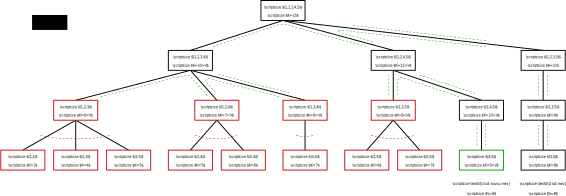
\includegraphics[width=\unitlength,page=1]{Branch_Bound.pdf}}%
    \put(0.024961,0.23201118){\color[rgb]{0,0,0}\makebox(0,0)[b]{\smash{}}}%
    \put(0.50000001,0.3170521){\color[rgb]{0,0,0}\makebox(0,0)[b]{\smash{\scriptsize $K=15$}}}%
    \put(0.69500781,0.22883558){\color[rgb]{0,0,0}\makebox(0,0)[b]{\smash{\scriptsize $K=12>V$}}}%
    \put(0.69500781,0.14061895){\color[rgb]{0,0,0}\makebox(0,0)[b]{\smash{\scriptsize $K=8<V$}}}%
    \put(0.85101402,0.14061895){\color[rgb]{0,0,0}\makebox(0,0)[b]{\smash{\scriptsize $K=10>V$}}}%
    \put(0.64820592,0.05240243){\color[rgb]{0,0,0}\makebox(0,0)[b]{\smash{\scriptsize $K=6$}}}%
    \put(0.74180964,0.05240243){\color[rgb]{0,0,0}\makebox(0,0)[b]{\smash{\scriptsize $K=7$}}}%
    \put(0.85101402,0.05240243){\color[rgb]{0,0,0}\makebox(0,0)[b]{\smash{\scriptsize $K=9>V$}}}%
    \put(0.96021839,0.05240243){\color[rgb]{0,0,0}\makebox(0,0)[b]{\smash{\scriptsize $K=8$}}}%
    \put(0.96021839,0.14061895){\color[rgb]{0,0,0}\makebox(0,0)[b]{\smash{\scriptsize $K=9$}}}%
    \put(0.96021839,0.22883558){\color[rgb]{0,0,0}\makebox(0,0)[b]{\smash{\scriptsize $K=11$}}}%
    \put(0.53900155,0.05240243){\color[rgb]{0,0,0}\makebox(0,0)[b]{\smash{\scriptsize $K=7$}}}%
    \put(0.53900155,0.14061895){\color[rgb]{0,0,0}\makebox(0,0)[b]{\smash{\scriptsize $K=8<V$}}}%
    \put(0.42979718,0.05240243){\color[rgb]{0,0,0}\makebox(0,0)[b]{\smash{\scriptsize $K=6$}}}%
    \put(0.33619345,0.05240243){\color[rgb]{0,0,0}\makebox(0,0)[b]{\smash{\scriptsize $K=5$}}}%
    \put(0.38299531,0.14061895){\color[rgb]{0,0,0}\makebox(0,0)[b]{\smash{\scriptsize $K=7<V$}}}%
    \put(0.33619345,0.22883558){\color[rgb]{0,0,0}\makebox(0,0)[b]{\smash{\scriptsize $K=10>V$}}}%
    \put(0.0397816,0.05240243){\color[rgb]{0,0,0}\makebox(0,0)[b]{\smash{\scriptsize $K=3$}}}%
    \put(0.13338534,0.05240243){\color[rgb]{0,0,0}\makebox(0,0)[b]{\smash{\scriptsize $K=4$}}}%
    \put(0.22698908,0.05240243){\color[rgb]{0,0,0}\makebox(0,0)[b]{\smash{\scriptsize $K=5$}}}%
    \put(0.13338534,0.14061895){\color[rgb]{0,0,0}\makebox(0,0)[b]{\smash{\scriptsize $K=6<V$}}}%
    \put(0.96021836,0.01940946){\color[rgb]{0,0,0}\makebox(0,0)[b]{\smash{\scriptsize \textit{Ulož mez}}}}%
    \put(0.96021836,0.00176607){\color[rgb]{0,0,0}\makebox(0,0)[b]{\smash{\scriptsize $V=8$}}}%
    \put(0.85101389,0.01940946){\color[rgb]{0,0,0}\makebox(0,0)[b]{\smash{\scriptsize \textit{Ulož novou mez}}}}%
    \put(0.85101389,0.00176607){\color[rgb]{0,0,0}\makebox(0,0)[b]{\smash{\scriptsize $V=9$}}}%
    \put(0.024961,0.24435908){\color[rgb]{0,0,0}\makebox(0,0)[b]{\smash{}}}%
    \put(0.5,0.33169359){\color[rgb]{0,0,0}\makebox(0,0)[b]{\smash{\scriptsize $(1,2,3,4,5)$}}}%
    \put(0.6950078,0.24347707){\color[rgb]{0,0,0}\makebox(0,0)[b]{\smash{\scriptsize $(1,2,4,5)$}}}%
    \put(0.6950078,0.15526044){\color[rgb]{0,0,0}\makebox(0,0)[b]{\smash{\scriptsize $(1,2,5)$}}}%
    \put(0.85101401,0.15526044){\color[rgb]{0,0,0}\makebox(0,0)[b]{\smash{\scriptsize $(1,4,5)$}}}%
    \put(0.64820591,0.06704393){\color[rgb]{0,0,0}\makebox(0,0)[b]{\smash{\scriptsize $(1,5)$}}}%
    \put(0.74180964,0.06704393){\color[rgb]{0,0,0}\makebox(0,0)[b]{\smash{\scriptsize $(2,5)$}}}%
    \put(0.85101401,0.06704393){\color[rgb]{0,0,0}\makebox(0,0)[b]{\smash{\scriptsize $(4,5)$}}}%
    \put(0.96021838,0.06704393){\color[rgb]{0,0,0}\makebox(0,0)[b]{\smash{\scriptsize $(3,5)$}}}%
    \put(0.96021838,0.15526044){\color[rgb]{0,0,0}\makebox(0,0)[b]{\smash{\scriptsize $(1,3,5)$}}}%
    \put(0.96021838,0.24347707){\color[rgb]{0,0,0}\makebox(0,0)[b]{\smash{\scriptsize $(1,2,3,5)$}}}%
    \put(0.53900154,0.06704393){\color[rgb]{0,0,0}\makebox(0,0)[b]{\smash{\scriptsize $(3,4)$}}}%
    \put(0.53900154,0.15526044){\color[rgb]{0,0,0}\makebox(0,0)[b]{\smash{\scriptsize $(1,3,4)$}}}%
    \put(0.42979717,0.06704393){\color[rgb]{0,0,0}\makebox(0,0)[b]{\smash{\scriptsize $(2,4)$}}}%
    \put(0.33619345,0.06704393){\color[rgb]{0,0,0}\makebox(0,0)[b]{\smash{\scriptsize $(1,4)$}}}%
    \put(0.38299531,0.15526044){\color[rgb]{0,0,0}\makebox(0,0)[b]{\smash{\scriptsize $(1,2,4)$}}}%
    \put(0.33619345,0.24347707){\color[rgb]{0,0,0}\makebox(0,0)[b]{\smash{\scriptsize $(1,2,3,4)$}}}%
    \put(0.03978159,0.06704393){\color[rgb]{0,0,0}\makebox(0,0)[b]{\smash{\scriptsize $(1,2)$}}}%
    \put(0.13338533,0.06704393){\color[rgb]{0,0,0}\makebox(0,0)[b]{\smash{\scriptsize $(1,3)$}}}%
    \put(0.22698908,0.06704393){\color[rgb]{0,0,0}\makebox(0,0)[b]{\smash{\scriptsize $(2,3)$}}}%
    \put(0.13338533,0.15526044){\color[rgb]{0,0,0}\makebox(0,0)[b]{\smash{\scriptsize $(1,2,3)$}}}%
  \end{picture}%
\endgroup%
